% !TeX program = xelatex
% !TeX encoding = UTF-8
% !TeX root = document.tex

% Command to compile document
% xelatex -synctex=1 -interaction=nonstopmode document.tex

% Recomended IDE is TeXstudio (https://texstudio.org/) 
% or another one, that supports magic comments

% Document class repo 
% https://github.com/mirea-ninja/Latex-Template-for-Report-Diploma-Thesis/

\documentclass{mirea}

\usepackage{array}
\usepackage{longtable}
\usepackage{float}

\usepackage{booktabs}


\usepackage{hyperref}
\hypersetup{pdftitle={Архитектура вычеслительных систем}, pdfauthor={В. С. Верхотуров}}

\usepackage{graphicx}

\begin{document}
	
	\begin{titlepage}
		
		\pagestyle{empty}
		
		\setlength\parindent{0pt}
		\newcommand{\blankDate}[2]{\mbox{\uline{<<\makebox[.7cm]{#1}>>~\makebox[2cm]{#2}~\the\year{}~г.}}} % {день}{месяц}
		\newcommand\blankLine[2]{$\underset{\text{#1}}{\text{\uline{#2}}}$}
		\begin{center}
			\includegraphics[width=2.5cm]{MIREA_Gerb_Black} \par
			МИНОБРНАУКИ РОССИИ \par 
			Федеральное государственное бюджетное образовательное учреждение высшего образования \par
			\textbf{<<МИРЭА~--- Российский технологический университет>>} \par
			\textbf{\fontsize{16pt}{16pt}\selectfont РТУ МИРЭА} \par
			\blankLine{(наименование института, филиала)}{Институт кибербезопасности и цифровых технологий} \par
			\blankLine{(наименование кафедры)}{Кафедра КБ-14 <<Цифровые технологии обработки данных>>} \par
			\vspace*{1cm}
			{\fontsize{16pt}{16pt}\selectfont
				\textbf{Доклад. Оценка производительности Docker контейнеров и виртуальных машин}} \par
			по дисциплине \blankLine{(наименование дисциплины)}{Архитектура вычеслительных систем}
		\end{center}
		Студент группы \blankLine{учебная группа, фамилия, имя, отчество студента}{БСМО-31-24 В.~С.~Верхотуров}\par
		\begin{center}
			\vfill Москва~--- \the\year{}~г.
		\end{center}
	\end{titlepage}
	\addtocounter{page}{3}
	
	
	\tableofcontents
	
	
	\section{Введение}
	
	В последние годы внимание к облачным вычислениям растет. ИТ-индустрия разработала множество технологий на основе Xen, HyperV, VMware vSphere, KVM и т.д., которые известны как технологии виртуализации. Для развертывания множества приложений на одной виртуальной машине приложения и зависимости должны быть организованы и изолированы. Благодаря виртуализации несколько приложений могут работать на одном физическом оборудовании. Недостатки технологий виртуализации: виртуальные машины большие по размеру, нестабильная производительность из-за работы нескольких виртуальных машин, процесс запуска занимает много времени, и виртуальные машины не могут решить проблемы, такие как управление, обновление программного обеспечения и непрерывная интеграция/доставка. Эти проблемы привели к появлению нового процесса, называемого контейнеризацией, что, в свою очередь, привело к виртуализации на уровне ОС, тогда как виртуализация приводит к поглощению на уровне оборудования. Контейнеризация использует операционную систему хоста, которая делит соответствующие библиотеки и ресурсы. Она более эффективна, потому что отсутствует гостевая ОС. На ядре хост-системы могут обрабатываться специфичные для приложения бинарные и библиотечные файлы, что делает выполнение очень быстрым. Контейнеры создаются с помощью платформы Docker, которая объединяет приложения и их зависимости. Эти контейнеры всегда выполняются в изолированном пространстве поверх ядра операционной системы. Эта функция контейнеризации Docker обеспечивает поддержку любого связанного приложения \cite{cit1}.
	
	В данной работе для количественной оценки и сравнения приложений на основе гипервизоров и Docker контейнеров проведена серия экспериментов. Эти тесты помогают понять последствия производительности двух основных технологий виртуализации — контейнеров и гипервизоров. Статья организована следующим образом: в разделе 2 представлено исследование фона и краткое объяснение технологий и платформ. Раздел 3 посвящен методологии, используемой для понимания сравнения производительности. В разделе 4 представлены результаты бенчмаркинга. Наконец, в разделе 5 приведены заключение и планы на будущее.
	
	
	
	\section{Исследование}
	
	\subsection{Docker}
	
	Контейнеризация — это технология, которая объединяет приложение, связанные зависимости и системные библиотеки, организованные в виде контейнера. Приложения, которые созданы и организованы, могут быть выполнены и развернуты как контейнер. Эта платформа называется Docker, она обеспечивает работу приложения в любой среде. Она также автоматизирует приложения, которые будут развернуты в контейнеры. Docker добавляет дополнительный уровень движка развертывания поверх контейнерной среды, где выполняются и виртуализируются приложения. Docker помогает обеспечить быструю и легковесную среду для эффективного выполнения кода. Четыре основные части Docker: Docker Контейнеры, Docker Клиент-Сервер, Docker Образы и Docker Движок. В следующих разделах будет подробное объяснение этих компонентов.
	
	\subsubsection{Docker Движок}
	
	Основная часть системы Docker — это Docker Движок, клиент-серверное приложение, установленное на хост-машине с следующими компонентами.
	(a) Docker Демон: тип долгоживущей программы (команда dockerd), которая помогает создавать, строить и запускать приложения.
	(b) REST API используется для связи с Docker демоном.
	(c) Клиент отправляет запрос к Docker демону через терминал для доступа к операциям.
	
	
	\begin{figure}[H]
		\centering
		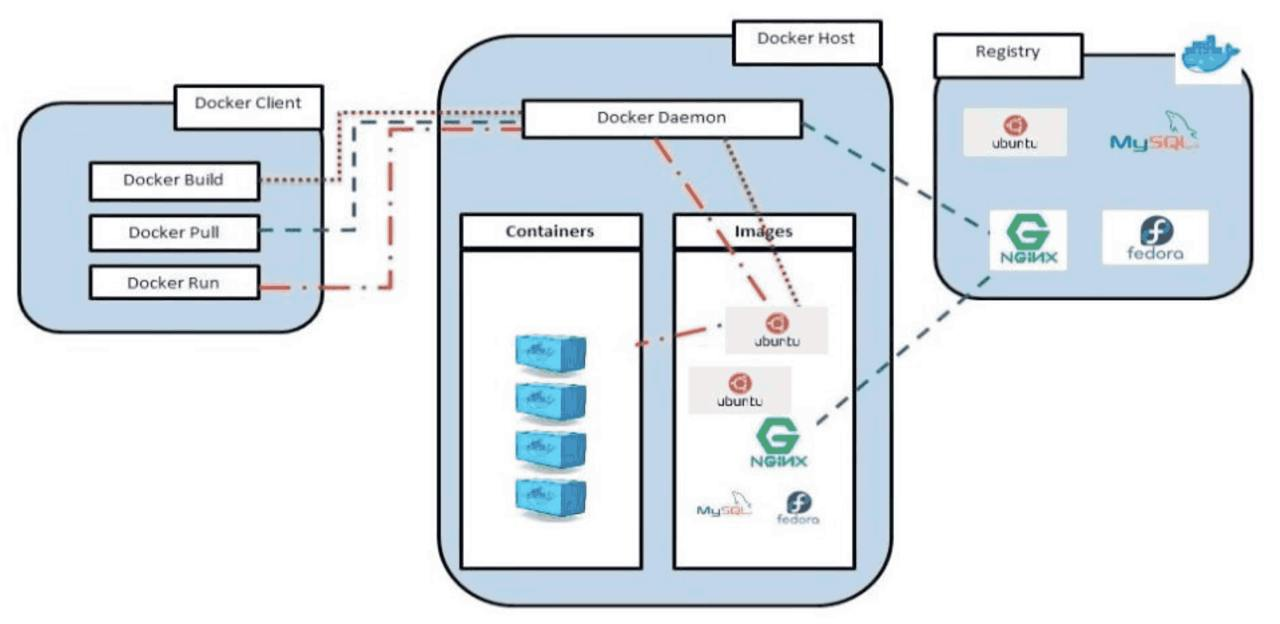
\includegraphics[width=\textwidth]{img1}
		\parskip=6pt
		\caption{Архитектура Docker Контейнера}
		\label{fig:pic1}
	\end{figure}

	\begin{figure}[H]
		\centering
		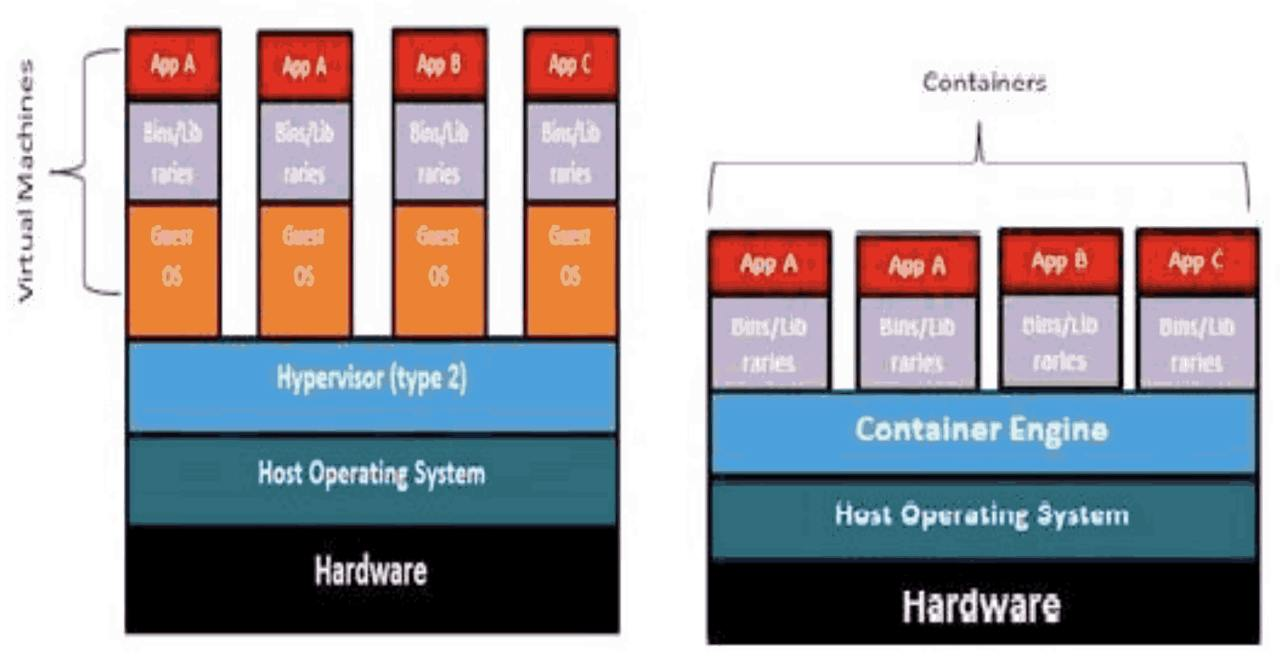
\includegraphics[width=\textwidth]{img2}
		\parskip=6pt
		\caption{(a) Архитектура на основе гипервизора (b) Архитектура на основе контейнеров}
		\label{fig:pic2}
	\end{figure}

	\subsubsection{Docker Клиент-Сервер}
	
	Технология Docker в основном относится к клиент-серверной архитектуре. Клиент связывается с Docker демоном, который выступает в роли сервера, находящегося внутри хост-машины. Демон работает как три основных процесса: запуск, построение и распространение контейнеров. Оба Docker контейнера и демон могут быть размещены на одной машине. Рис. 1. показывает архитектуру Docker.
	
	\subsubsection{Docker Образы}
	
	Docker Образы могут быть созданы двумя методами. Основной метод — построение образа с помощью шаблона только для чтения. Шаблон состоит из базовых образов, это может быть операционная система, такая как CentOs, Ubuntu, Fedora или любые другие базовые образы ОС, которые являются легковесными. Обычно базовые образы являются основой каждого образа. Необходимо создавать новый образ каждый раз, когда базовые образы создаются с нуля. Этот тип создания нового образа называется "фиксацией изменений". Следующий метод — создание Docker файла, который содержит все инструкции для создания Docker образа. Когда команда docker build выполняется из терминала, образ будет создан со всеми зависимостями, указанными в Docker файле. Этот процесс называется автоматизированным методом создания образа.
	
	\subsubsection{Docker Контейнеры}
	
	Docker Контейнеры создаются из Docker Образа. Для выполнения приложения в ограниченной среде контейнер должен содержать все необходимые компоненты для приложения. Образы контейнеров могут быть созданы на основе требований сервиса для приложения или программного обеспечения. Предположим, что приложение, включающее ОС Ubuntu и сервер Nginx, должно быть добавлено в Dockerfile. Используя команду "docker run", создается контейнер с образом ОС Ubuntu, включающим сервер Nginx, и начинает работать.
	
	\subsubsection{Сравнение Виртуальной Машины и Docker Контейнера}
	
	Docker иногда называют легковесными ВМ, но они не являются ВМ. Основная технология, как показано в таблице 1 ниже, различается в технологиях виртуализации. Рис. \ref{fig:pic2}. показывает архитектуру виртуальной машины и Docker контейнера.
	
	\begin{table}[h]
		\centering
		\caption{Сравнение Виртуальных Машин и Docker Контейнеров}
		\begin{tabular}{@{}p{4cm}p{4cm}p{4cm}@{}}
			\toprule
			& Виртуальные Машины & Docker Контейнеры \\ \midrule
			Изоляция на уровне процесса & Оборудование & Операционная Система \\
			Операционная Система & Разделена & Общая \\
			Время запуска & Долгое & Короткое \\
			Использование ресурсов & Больше & Меньше \\
			Предварительно созданные образы & Трудно найти и управлять & Уже доступны для домашнего сервера \\
			Настраиваемые предварительно настроенные образы & Трудно создавать & Легко создавать \\
			Размер & Больше, так как содержат всю ОС & Меньше, только с Docker движками поверх хост ОС \\
			Мобильность & Легко перемещать на новую хост ОС & Уничтожаются и создаются заново вместо перемещения \\
			Время создания & Дольше & В течение нескольких секунд \\ 
			\bottomrule
		\end{tabular}
	\end{table}

	\subsection{Связанные работы}
	
	Использование виртуальных машин (ВМ) распространено в организациях. ВМ широко используются для выполнения сложных задач, таких как Hadoop \cite{cit2}. Однако пользователи также используют ВМ даже для запуска небольших приложений, что делает систему неэффективной. Существует необходимость в запуске легковесного приложения, которое работает быстрее и делает систему эффективной. Docker контейнер — одна из технологий, предлагающих легковесную виртуализацию, и это мотивирует нас провести исследование фона. Рис. \ref{fig:pic1}. иллюстрирует архитектуру Docker Контейнера.
	
	В \cite{cit3} авторы представляют обзор оценки производительности виртуальных машин и Docker контейнеров в терминах производительности ЦП, пропускной способности памяти, ввода/вывода диска и измерения скорости операций. Авторы в \cite{cit4} сосредоточились на внедрении Docker контейнеров в HPC кластер. В последней части статьи авторы объясняют различные подходы к выбору модели контейнера и использованию LNPACK и BLAS. В \cite{cit5} авторы обсуждают легковесные подходы к виртуализации, в которых рассматриваются проблемы контейнеров и unikernel. Далее в статье также обсуждается статистическая оценка ANOVA теста и пост-хок сравнение с использованием метода Tukey собранных данных. Автор также обсуждает различные инструменты бенчмаркинга, используемые для сравнения unikernel и контейнеров. Статический HTTP сервер и параметры хранилища ключ-значение используются для экспериментального анализа производительности приложений, развернутых в облаке. Сервер Nginx используется для производительности HTTP, а для измерения операций get и set используется Redis benchmark.
	
	Авторы в \cite{cit6} обсуждают оценку с использованием бенчмарк-приложений с KVM, Docker и OSv. В \cite{cit7} авторы обсуждают краткий обзор виртуальных машин и контейнерных технологий. Также обсуждается Docker и производительность Docker с различными параметрами ЦП, пропускной способности памяти, ввода/вывода диска. В \cite{cit8} автор обсуждает основные концепции архитектуры Docker, компоненты Docker, Docker образы, Docker реестры, архитектуру клиента и сервера Docker. Различия между виртуальными машинами и Docker контейнерами обсуждаются. В \cite{cit9} авторы объясняют сравнение производительности контейнерных технологий для облака с различным набором параметров. В статье представлена информация об использовании облачных развертываний на основе OpenStack, которые рассматриваются для сравнения. Платформы, используемые для сравнения производительности, — это Docker, LXC и flockport. Авторы в \cite{cit10} обсуждают сравнение производительности виртуальных машин и Docker по различным параметрам, таким как ЦП, сеть, диск и два реальных серверных приложения, Redis и MySql.
	
	\section{Методология}
	
	\begin{figure}[H]
		\centering
		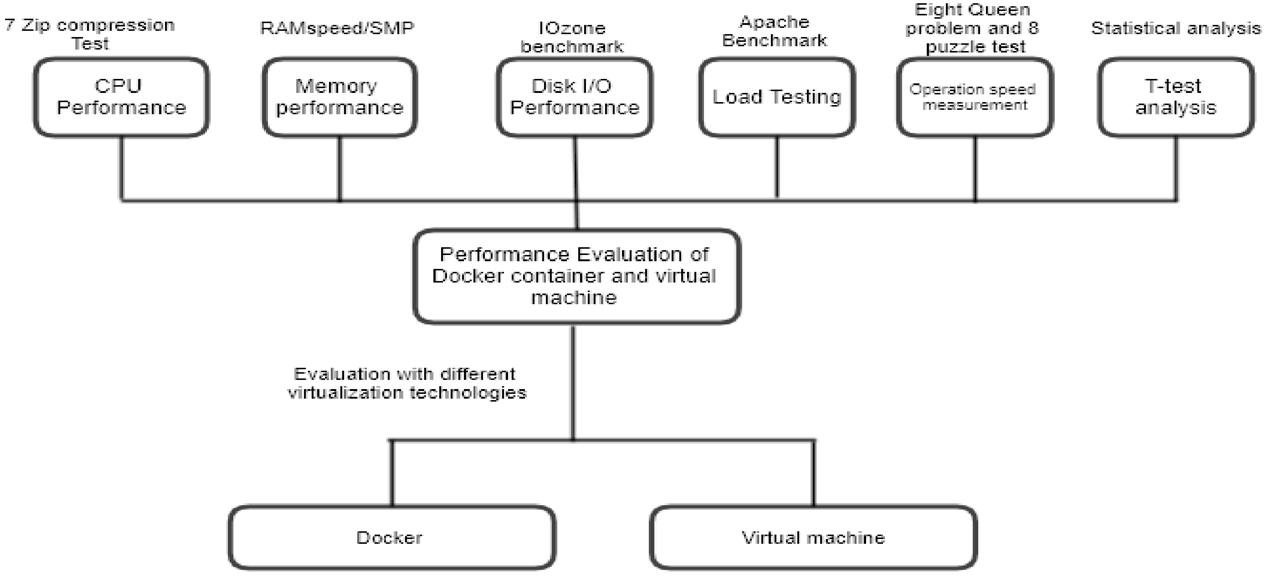
\includegraphics[width=.7\textwidth]{img3}
		\parskip=6pt
		\caption{Оценка производительности с использованием различных инструментов бенчмаркинга}
		\label{fig:pic3}
	\end{figure}
	
	
	В этом разделе оцениваются KVM и Docker с использованием инструментов бенчмаркинга. Следующие инструменты бенчмаркинга используются для оценки производительности: Sysbench \cite{cit11}, Phoronix \cite{cit12}, Apache benchmark \cite{cit13}. Эти инструменты бенчмаркинга измеряют производительность ЦП, пропускную способность памяти, производительность чтения и записи на диск, нагрузочное тестирование и измерение скорости операций. Для оценки производительности по различным параметрам используются два сервера HP, один из которых используется как виртуальная машина, установленная поверх хост ОС (Windows 10), а гостевая ОС (Ubuntu 20.04) с дополнением Docker движка, установленного поверх виртуальной машины, и другой сервер как bare metal с хост ОС Ubuntu 20.04 и Docker движком, установленным на нем. Все тесты проводились на сервере HP с двумя процессорами Intel Xenon E5-2620 v3 на частоте 2,40 ГГц с общей мощностью 12 ядер и 64 ГБ ОЗУ. Ubuntu 16.04 64-bit с ядром Linux 3.10.0 использовалась для выполнения всех тестов. Для поддержания согласованности и единообразия использовалась одна и та же операционная система, Ubuntu 20.04, в качестве базового образа для всех Docker контейнеров. Для ВМ настроено 12 vCPU и достаточно ОЗУ. Рис. \ref{fig:pic3}. представляет методологию оценки различных технологий виртуализации с использованием различных инструментов бенчмаркинга.
	
	\section{Результаты и обсуждения}
	
	В этом разделе обсуждается анализ производительности технологий виртуализации. Результаты классифицируются на четыре подраздела. Раздел 4.1 описывает все измерения ЦП; пропускная способность памяти показана в разделе 4.2; измерения чтения и записи на диск показаны в разделах 4.3. Раздел 4.4 представляет анализ нагрузочного тестирования. Раздел 4.5 описывает измерение скорости операций, которое включает два теста: задача восьми ферзей и задача восьми пазлов.
	
	\subsection{Производительность ЦП}
	
	Вычислительная производительность может быть измерена количеством операций, выполненных системой в течение определенного времени (событий/сек) или временем выполнения определенной задачи. Результаты в основном зависят от количества виртуальных ядер ЦП, выделенных серверу. Сравнение производительности ЦП проводилось с использованием следующих инструментов: sysbench, Phoronix и Apache benchmark.
	
	\subsubsection{Максимальная операция с простыми числами}
	
	На инструменте Sysbench проведен тест для определения времени, необходимого для выполнения операции с максимальным простым числом. Максимальное значение простого числа для операции взято равным 50000 с временем 60 секунд и 4 потоками операций. На рис. \ref{fig:pic4}. видно, что Docker контейнер выполняет операцию значительно быстрее по сравнению с ВМ. Это связано с наличием гипервизора в виртуальной машине. Поэтому для выполнения требуется больше времени.
	
	\begin{figure}[H]
		\centering
		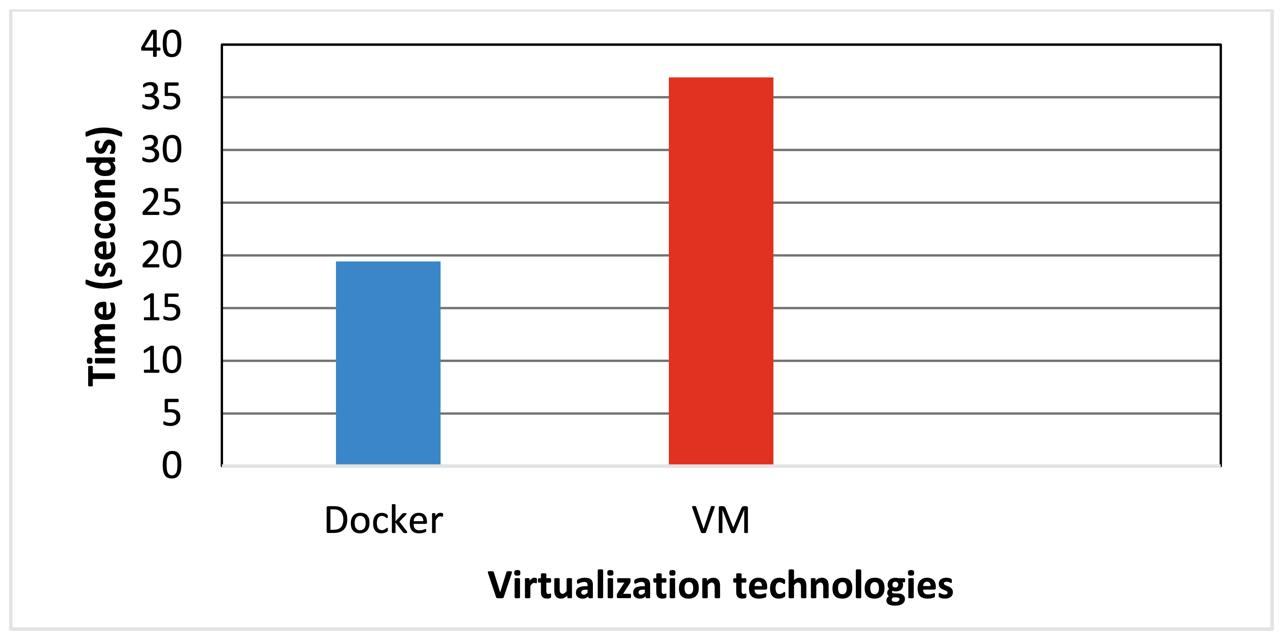
\includegraphics[width=.6\textwidth]{img4}
		\parskip=6pt
		\caption{Сравнение производительности ЦП Docker и виртуальной машины}
		\label{fig:pic4}
	\end{figure}

	\subsubsection{Тест на Сжатие 7 Zip}
	
	7-Zip — это архиватор с открытым исходным кодом, который используется для сжатия группы файлов в контейнеры, называемые "архивами". Два теста для LZMA бенчмарка: сжатие и декомпрессия методов LZMA. Этот тест измеряет время, необходимое для сжатия файла с использованием сжатия 7 Zip. Размер файла, используемого для теста сжатия, составляет 10 ГБ. Рис. \ref{fig:pic5}. показывает сравнение производительности ЦП с тестом на сжатие 7 Zip. Таким образом, согласно полученным результатам, производительность Docker Контейнера значительно лучше, чем у ВМ при выполнении сжатия большого количества файлов.
	
	\begin{figure}[H]
		\centering
		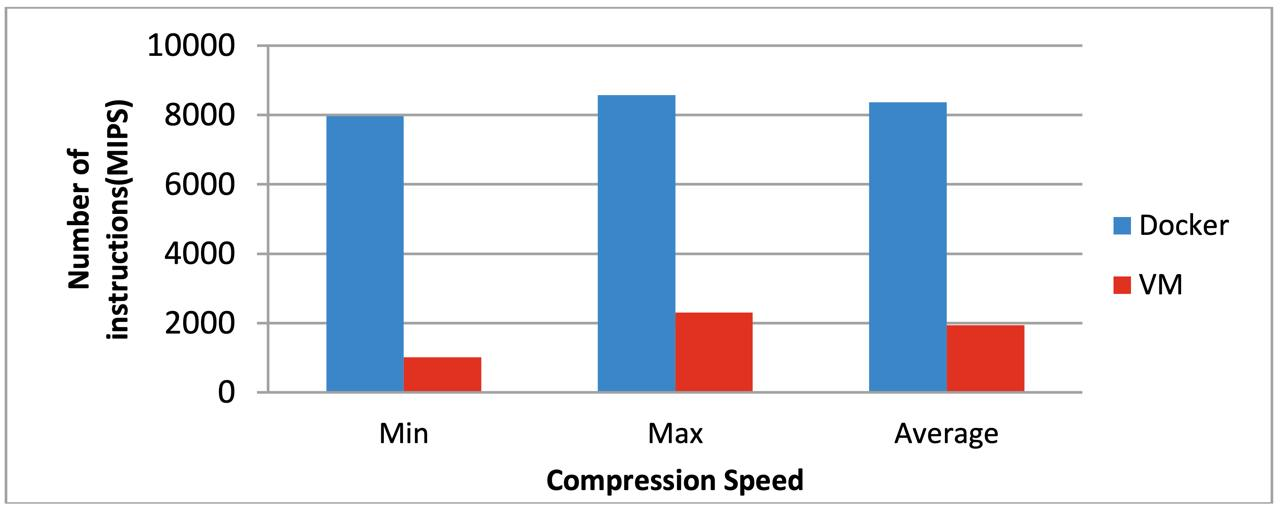
\includegraphics[width=.6\textwidth]{img5}
		\parskip=6pt
		\caption{Тест на сжатие для производительности ЦП}
		\label{fig:pic5}
	\end{figure}

	\subsection{Производительность памяти}
	
	RAM speed/SMP (Symmetric Multiprocessing) — это инструмент для бенчмаркинга кэша и памяти, используемый для измерения скорости RAM для технологий виртуализации, то есть Docker и Виртуальной Машины. Рис. 6. представляет сравнение скорости RAM между технологиями виртуализации. При тестировании скорости RAM учитывались следующие два основных параметра. Компоненты INTmark и FLOATmark используются в инструменте бенчмаркинга RAM Speed SMP, который измеряет максимально возможную производительность кэша и памяти при чтении и записи отдельных блоков данных.
	
	INTmem и FLOATmem — это синтетические симуляции, но они тесно связаны с реальным миром вычислений. Каждая из них состоит из четырех подтестов (Copy, Scale, Add, Triad) для измерения различных аспектов производительности памяти. Команда copy передает данные из одного места памяти в другое, то есть (X=Y). Команда scale изменяет данные перед записью, умножая их на определенное постоянное значение, то есть (X=n*Y). Команда ADD читает данные из первого места памяти, затем из второго, когда вызывается, и помещает результирующие данные в третье место (X=Y+Z). Triad — это комбинация Add и Scale. Данные читаются из первого места памяти для масштабирования, затем добавляются из второго места для записи в третье место (X=n*Y+Z). Рис. \ref{fig:pic6}. показывает производительность памяти в зависимости от теста RAM Speed SMP.
	
	\begin{figure}[H]
		\centering
		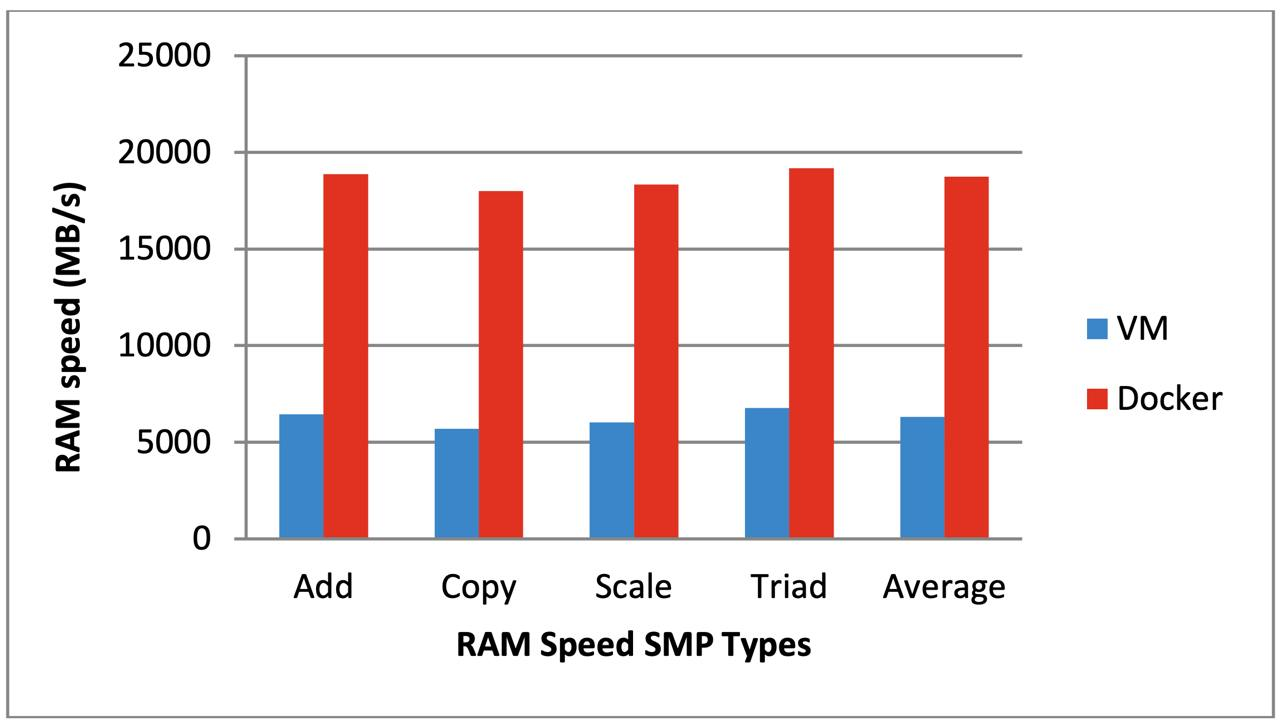
\includegraphics[width=.6\textwidth]{img6}
		\parskip=6pt
		\caption{Сравнение скорости RAM между технологиями виртуализации}
		\label{fig:pic6}
	\end{figure}

	\subsection{Производительность ввода/вывода на диск}
	
	Для тестирования производительности жесткого диска используется инструмент бенчмаркинга IOzone. Для тестирования операций чтения и записи системы использовался размер записи 1 МБ и размер файла 4 ГБ. Можно сделать вывод из рис. 7, что производительность Docker значительно лучше по сравнению с виртуальной машиной. Операции записи и чтения на диск ВМ уменьшены более чем вдвое по сравнению с Docker контейнером (примерно на 54\%). Рис. \ref{fig:pic7}. показывает производительность диска как виртуальных машин, так и Docker.
	
	\begin{figure}[H]
		\centering
		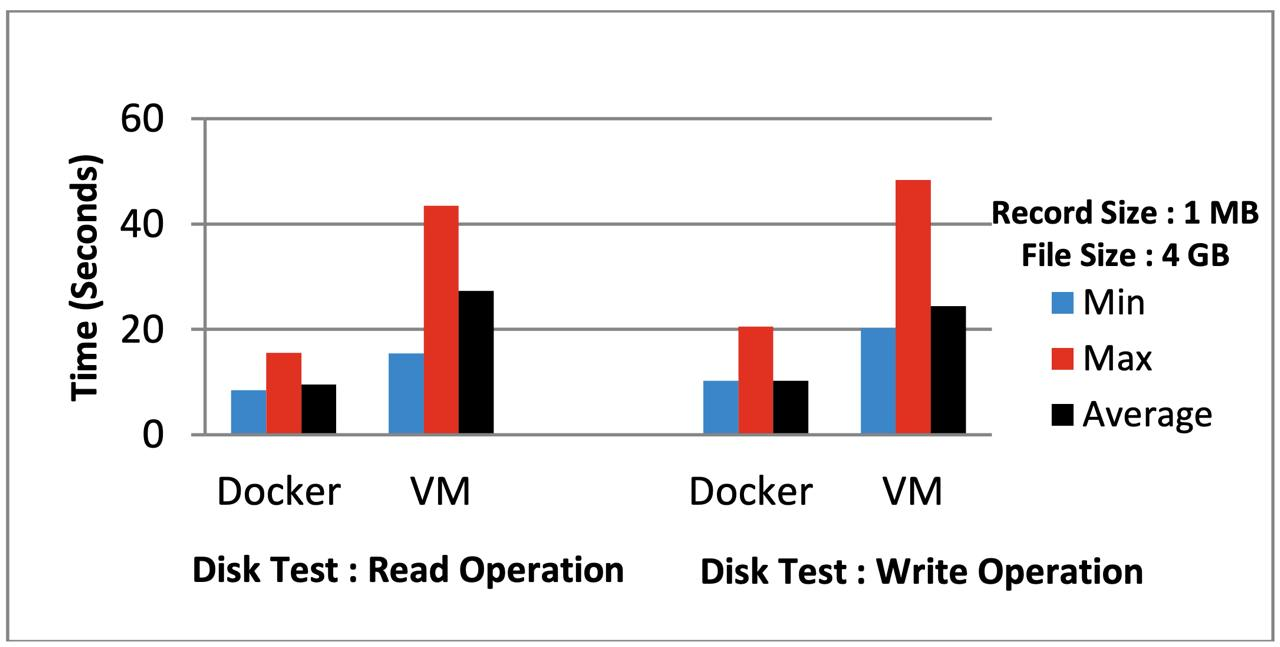
\includegraphics[width=.6\textwidth]{img7}
		\parskip=6pt
		\caption{Производительность диска по IOzone Benchmark}
		\label{fig:pic7}
	\end{figure}

	\subsection{Нагрузочное тестирование}
	
	Для сравнения производительности нагрузочного тестирования используется инструмент Apache Benchmark, который измеряет количество запросов в секунду, которое может выдержать данная система. Программа на Python выполняется для тестирования нагрузки с использованием инструмента Apache Benchmark. Рис. \ref{fig:pic8}. показывает, что пропускная способность для ВМ значительно ниже по сравнению с Docker. Это связано с более высокой сетевой задержкой в виртуальной машине по сравнению с Docker. Анализ показывает, что Docker контейнер лучше справляется с количеством запросов в секунду по сравнению с виртуальной машиной.
	
	\begin{figure}[H]
		\centering
		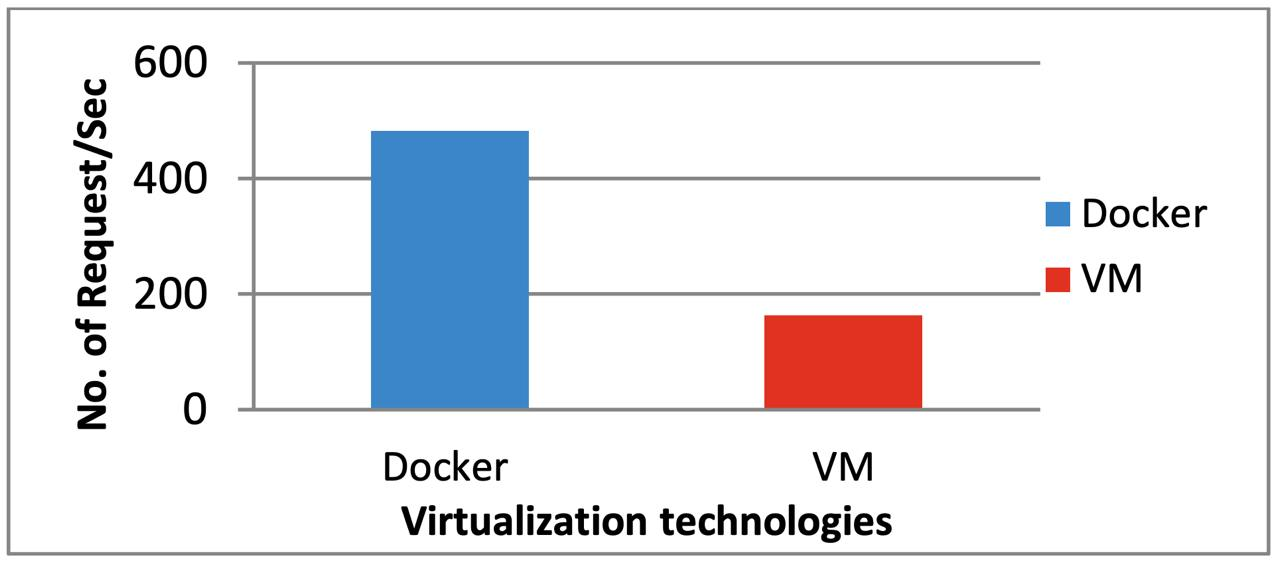
\includegraphics[width=.6\textwidth]{img8}
		\parskip=6pt
		\caption{Сравнение нагрузочного тестирования между Docker и виртуальной машиной}
		\label{fig:pic8}
	\end{figure}

	\subsection{Измерение скорости операций}
	
	Задача восьми ферзей заключается в размещении восьми ферзей на шахматной доске 8x8 так, чтобы они не били друг друга. Тест измеряет, сколько времени требуется для решения задачи. Программа для восьми ферзей написана на Python и определяет вычислительную производительность системы. Рис. \ref{fig:pic9}. показывает вычислительную производительность как Docker, так и виртуальных машин. На основе времени выполнения Docker контейнер тратит меньше времени на решение задачи, тогда как виртуальная машина тратит гораздо больше времени.
	
	\begin{figure}[H]
		\centering
		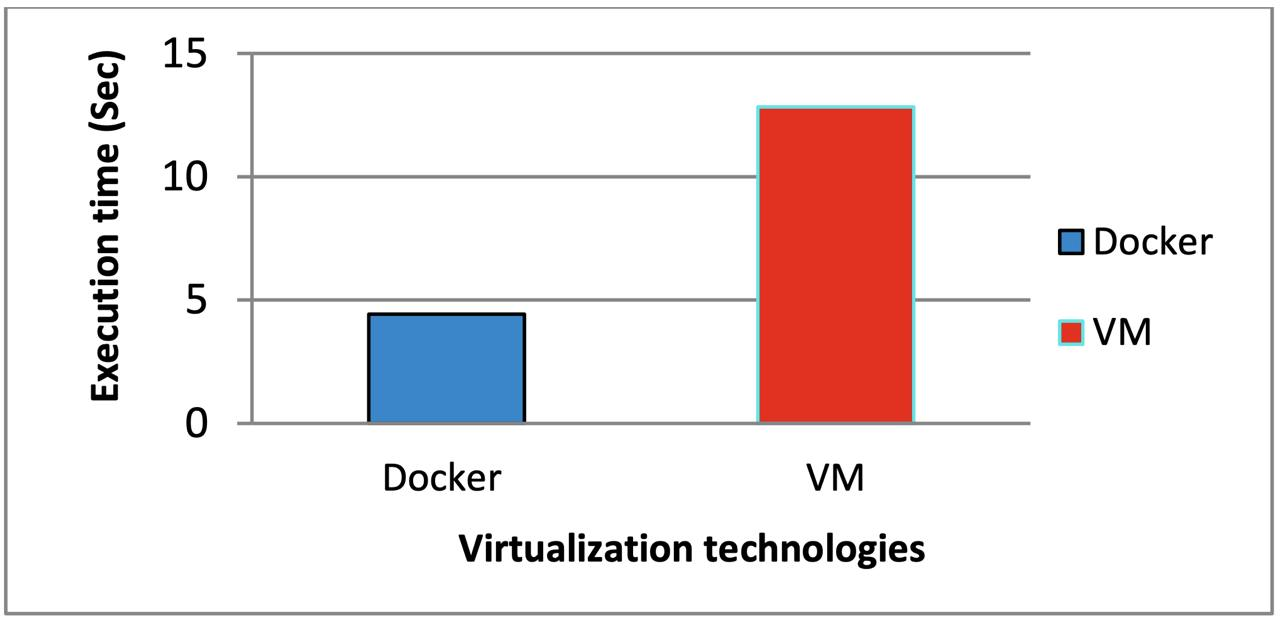
\includegraphics[width=.6\textwidth]{img9}
		\parskip=6pt
		\caption{Сравнение производительности программы для задачи восьми ферзей}
		\label{fig:pic9}
	\end{figure}

	Тест на восьми пазлах: используется доска 4x4 с 8 плитками и одним пустым местом. Используя пустое место, необходимо переместить количество плиток для соответствия конечной конфигурации. Можно сдвигать четыре смежные операции (вправо, влево, вниз и вверх) плитки на пустое место — тест измеряет, сколько времени требуется для решения задачи. Программа для восьми пазлов написана на Python и определяет вычислительную производительность системы. Рис. \ref{fig:pic10} показывает вычислительную производительность как Docker, так и виртуальных машин. На основе времени выполнения Docker контейнер тратит меньше времени на решение задачи, тогда как виртуальная машина тратит гораздо больше времени.
	
	\begin{figure}[H]
		\centering
		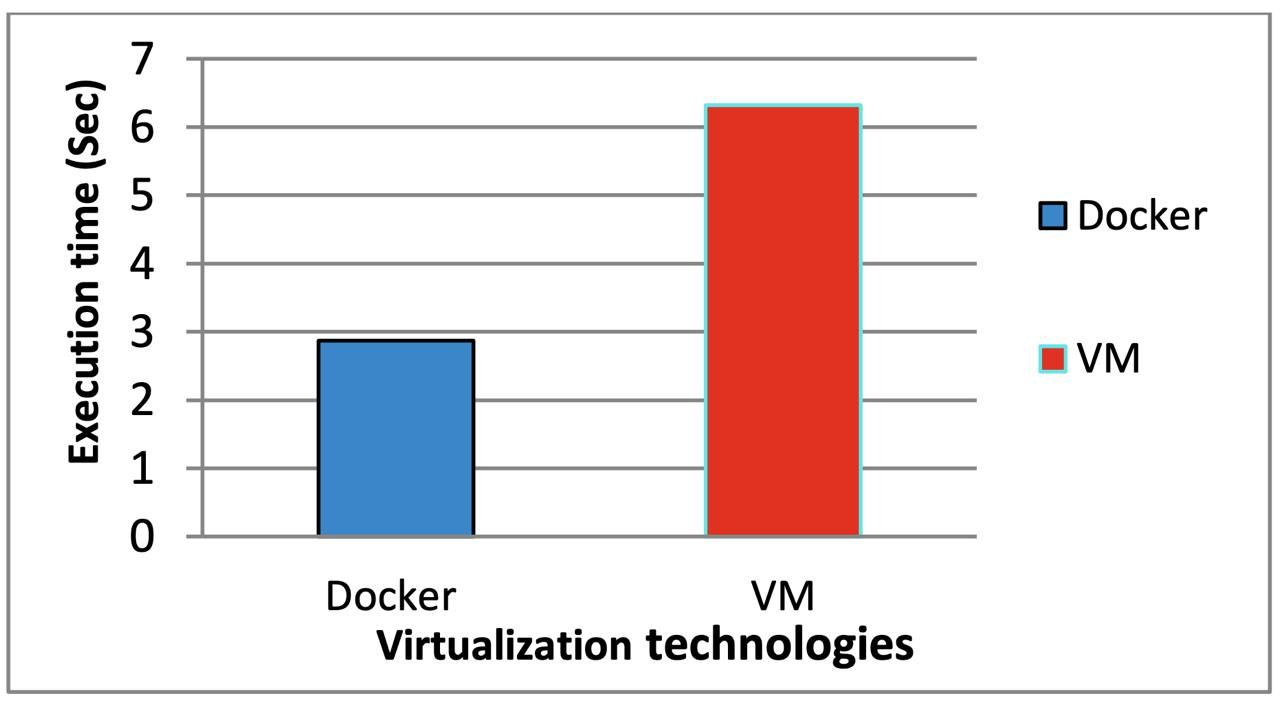
\includegraphics[width=.6\textwidth]{img10}
		\parskip=6pt
		\caption{Сравнение производительности теста на восьми пазлах}
		\label{fig:pic10}
	\end{figure}

	\section{Заключение}
	
	Docker Контейнер — это новая легковесная технология виртуализации. В данной работе оцениваются две технологии виртуализации, а именно Docker контейнеры и виртуальные машины. Оценка производительности проводится на хостах на основе виртуальных машин и Docker контейнеров в отношении производительности ЦП, пропускной способности памяти, ввода/вывода на диск, нагрузочного тестирования и измерения скорости операций. Наблюдается, что Docker контейнеры работают лучше, чем ВМ, в каждом тесте, так как наличие уровня QEMU в виртуальной машине делает ее менее эффективной по сравнению с Docker контейнерами. Оценка производительности как контейнеров, так и виртуальной машины проводится с использованием инструментов бенчмаркинга, таких как Sysbench, Phoronix и Apache benchmark.

	
	
	\begin{thebibliography}{99\kern\bibindent}
		\bibitem{cit1} Docker. https://docs.docker.com/
		\bibitem{cit2} Shivaraj Kengond, DG Narayan и Mohammed Moin Mulla (2018) "Hadoop как сервис в OpenStack" в Emerging Research in Electronics, Computer Science and Technology, стр. 223-233.
		\bibitem{cit3} C. G. Kominos, N. Seyvet и K. Vandikas, (2017) "Bare-metal, виртуальные машины и контейнеры в OpenStack" 20-я Конференция по Инновациям в Облаках, Интернете и Сетях (ICIN), Париж, стр. 36-43.
		\bibitem{cit4} Higgins J., Holmes V и Venters C. (2015) "Оркестрация Docker Контейнеров в HPC Среде". В: Kunkel J., Ludwig T. (ред.) Высокопроизводительные вычисления, Lecture Notes in Computer Science, том 9137, стр. 506-513
		\bibitem{cit5} Max Plauth, Lena Feinbube и Andreas Polze, (2017) "Оценка производительности легковесных подходов к виртуализации", CLOUD COMPUTING: Восьмая Международная Конференция по Облачным Вычислениям, GRIDs и Виртуализации.
		\bibitem{cit6} Kyoung-Taek Seo, Hyun-Seo Hwang, Il-Young Moon, Oh-Young Kwon и Byeong-Jun Kim "Сравнительный анализ производительности Linux Контейнера и Виртуальной Машины для построения облака," Advanced Science and Technology Letters Vol.66, стр. 105-111.
		\bibitem{cit7} R. Morabito, J. Kjällman и M. Komu, (2015) "Гипервизоры против легковесной виртуализации: сравнение производительности", Международная конференция IEEE по облачной инженерии, Темпе, АЗ, стр. 386-393.
		\bibitem{cit8} Babak Bashari Rad, Harrison John Bhatti и Mohammad Ahmadi (2017) "Введение в Docker и анализ его производительности" ECSNS International Journal of Computer Science and Network Security, VOL. 17 No.3, стр. 228-229.
		\bibitem{cit9} Kochirbayev, Zhanibek, и Richard O. Sinnott. (2017) "Сравнение производительности контейнерных технологий для облака", Future Generation Computer Systems, стр. 175-182.
		\bibitem{cit10} Felter, Wes, и др. (2015) "Сравнение производительности виртуальных машин и Linux контейнеров", Международный симпозиум IEEE по анализу производительности систем и программного обеспечения (ISPASS), стр. 171-172.
		\bibitem{cit11} Sysbench. https://wiki.gentoo.org/wiki/Sysbench 2019
		\bibitem{cit12} Инструмент бенчмаркинга Phoronix. https://www.phoronix-test-suite.com/
		\bibitem{cit13} Инструмент бенчмаркинга Apache. https://www.tutorialspoint.com/apache\_bench/
	\end{thebibliography}

	
	
	
	
	
	
	
\end{document}
